\documentclass[12pt]{article}
    \title{\textbf{Monitoraggio temperatura forno solare e controllo automatico orientamento specchi}}
    \author{Scar. Francesco}
    \date{}
    \addtolength{\topmargin}{-2cm}
    \addtolength{\textheight}{3cm}
    \renewcommand{\contentsname}{Contenuti}
    \newenvironment{changemargin}[2]{%
    \begin{list}{}{%
    \setlength{\topsep}{0pt}%
    \setlength{\leftmargin}{#1}%
    \setlength{\rightmargin}{#2}%
    \setlength{\listparindent}{\parindent}%
    \setlength{\itemindent}{\parindent}%
    \setlength{\parsep}{\parskip}%
    }%
    \item[]}{\end{list}}
    \long\def\/*#1*/{}          % Multiline comments https://tex.stackexchange.com/questions/87303/multi-line-block-comments-in-latex
    \usepackage{pdfpages}
    \usepackage{listings}
    \usepackage[utf8]{inputenc}
    \usepackage[T1]{fontenc}
    \usepackage{textcomp}
    \usepackage{gensymb}
    \usepackage{typearea}
    \usepackage[utf8]{inputenc}
    \usepackage[T1]{fontenc}
    \usepackage{color}
    \usepackage{mwe}
    \usepackage{listings}    
    \usepackage{etoolbox}    
    \usepackage{hyperref}
    \usepackage{amsmath}
    
    \definecolor{mygreen}{rgb}{0,0.6,0}
    \definecolor{mygray}{rgb}{0.47,0.47,0.33}
    \definecolor{myorange}{rgb}{0.8,0.4,0}
    \definecolor{mywhite}{rgb}{0.98,0.98,0.98}
    \definecolor{myblue}{rgb}{0.01,0.61,0.98}
    

    \newcommand*{\FormatDigit}[1]{\ttfamily\textcolor{mygreen}{#1}}
    %% https://tex.stackexchange.com/questions/32174/listings-package-how-can-i-format-all-numbers
    \lstdefinestyle{FormattedNumber}{%
        literate=*{0}{{\FormatDigit{0}}}{1}%
                 {1}{{\FormatDigit{1}}}{1}%
                 {2}{{\FormatDigit{2}}}{1}%
                 {3}{{\FormatDigit{3}}}{1}%
                 {4}{{\FormatDigit{4}}}{1}%
                 {5}{{\FormatDigit{5}}}{1}%
                 {6}{{\FormatDigit{6}}}{1}%
                 {7}{{\FormatDigit{7}}}{1}%
                 {8}{{\FormatDigit{8}}}{1}%
                 {9}{{\FormatDigit{9}}}{1}%
                 {.0}{{\FormatDigit{.0}}}{2}% Following is to ensure that only periods
                 {.1}{{\FormatDigit{.1}}}{2}% followed by a digit are changed.
                 {.2}{{\FormatDigit{.2}}}{2}%
                 {.3}{{\FormatDigit{.3}}}{2}%
                 {.4}{{\FormatDigit{.4}}}{2}%
                 {.5}{{\FormatDigit{.5}}}{2}%
                 {.6}{{\FormatDigit{.6}}}{2}%
                 {.7}{{\FormatDigit{.7}}}{2}%
                 {.8}{{\FormatDigit{.8}}}{2}%
                 {.9}{{\FormatDigit{.9}}}{2}%
                 %{,}{{\FormatDigit{,}}{1}% depends if you want the "," in color
                 {\ }{{ }}{1}% handle the space
                 ,%
    }


    \lstset{%
      backgroundcolor=\color{mywhite},   
      basicstyle=\footnotesize,       
      breakatwhitespace=false,         
      breaklines=true,                 
      captionpos=b,                   
      commentstyle=\color{gray},    
      deletekeywords={...},           
      escapeinside={\%*}{*)},          
      extendedchars=true,              
      frame=single,                    
      keepspaces=true,                 
      keywordstyle=\color{myorange},       
      language=c++,                
      morekeywords={*,...},            
      numbers=left,                   
      numberstyle=\tiny\color{mygray}, 
      rulecolor=\color{black},         
      rulesepcolor=\color{myblue},
      showspaces=false,                
      showstringspaces=false,          
      showtabs=false
      stringstyle=\color{green},    
      tabsize=2,
      emphstyle=\bfseries\color{blue},%  style for emph={} 
    }    

    %% language specific settings:
    \lstdefinestyle{Arduino}{%
        style=FormattedNumber,
        keywords={void},%                 define keywords
        morecomment=[l]{//},%             treat // as comments
        morecomment=[s]{/*}{*/},%         define /* ... */ comments
        emph={HIGH, OUTPUT, LOW},%        keywords to emphasize
    }

    \newtoggle{InString}{}% Keep track of if we are within a string
    \togglefalse{InString}% Assume not initally in string
\begin{document}


\maketitle

\tableofcontents{}

\newpage

%\vfill


\section{Introduzione}
    \subsection{Descrizione}
    Si desidera realizzare un sistema di controllo automatico dell'orientamento e inclinazione degli specchi di un forno solare per garantire la massima efficienza al variare della posizione relativa del sole nell'arco della giornata.
    Si desidera inoltre monitorare la temperatura e lo stato di funzionamento generale del sistema mediante un'interfaccia web che permetta l'impostazione di notifiche di allarme in caso di una temperatura troppo bassa per un tempo prolungato oppure trascorso un tempo prestabilito (funzione "timer").

\section{Schema a blocchi}

\/*
\noindent
\includegraphics[
    page=1,
    width=\textwidth,
    height=\textheight,
    keepaspectratio
]{}
*/


\vspace{0.5cm}
\noindent


%Text below%\footnotemark[1]

\vfill



\section{Descrizione componenti}
    \subsection{Microcontrollore}
    Per la realizzazione di questo sistema di controllo è stato scelto di utilizzare un ESP-32, un microcontrollore a 32 bit con ingressi e uscite compatibili con la logica TTL.\\
    Per semplicità costruttiva di seguito ci si riferirà alla specifica implementazione me\-dian\-te la scheda di prototipazione rapida Arduino UNO.
    \subsection{Motori}
    Si assume che l'apertura e la chiusura dei pannelli che costituiscono il tetto siano realiz\-zate attraverso l'attivazione di un motore in continua a 12V (potenza 25W), che, ad esempio, mediante un sistema vite-dado permette di trasformare il movimento rotatorio del motore in un movimento lineare; chiaramente l'apertura avviene grazie alla rotazione in un senso dell'asse del motore (si supponga in verso orario), mentre la chiusura avviene con la rotazione di senso opposto (antiorario).
        \subsubsection{Controllo di potenza}
        Dovendo controllare la direzione di rotazione del motore è necessaria la realizzazione di ponte H, di seguito un esempio di costruzione con transistor MOSFET.\\

        \vspace{0.1cm}


    \subsection{Sensori di temperatura}
    Per la rilevazione della temperatura si è scelto di utilizzare il sensore LM35 che fornisce un'uscita in tensione proporzionale alla temperatura (in °C) ed è utilizzabile, nella con\-fi\-gu\-ra\-zio\-ne base, in un range di temperature da 2°C a 150°, in cui rientrano ampiamente le temperature tipiche di una serra.\\
    La tensione fornita in uscita del sensore è legata alla temperatura $T$ in gradi Celsius dalla relazione:
    \begin{equation}
        V_{out} = T \cdot 10 \frac{mV}{\degree C}
    \end{equation}
    È stato scelto di condizionare ogni segnale separatamente per ridurre le distorsioni re\-la\-ti\-ve dei segnali, dovute alla trasmissione via cavo per relativamente lunghe distanze causate dalla disposizione dei sensori all'interno della serra; infatti a parità di rumore assoluto il rapporto segnale-rumore è maggiore, e quindi migliore, per segnali a tensioni maggiori.\\
    Il costruttore del sensore, nel datasheet, garantisce una precisione inferiore a 0.5°C (sti\-ma\-to per eccesso), questo comporta una possibile escursione dell'uscita del sensore cor\-ris\-pon\-den\-te alla variazione di $\pm$0.5°C anche in condizioni di temperatura stazionaria, per questo motivo è opportuno gestire la possibile oscillazione della temperatura nell'al\-go\-rit\-mo decisionale, creando un'isteresi di $\pm$0.5°C nell'intorno della soglia T, per evitare indesiderate e ripetute aperture e chiusure dei pannelli della serra che possono dan\-neg\-gia\-re i componenti meccanici, oltre ad aumentare i consumi e a produrre altri effetti indesiderati.
    
    \subsection{Display}
    Per la visualizzazione delle temperature è stato scelto l'utilizzo di un display LCD con 16x2 caratteri e interfaccia I$^2$C, che permette la comunicazione attraverso due soli se\-gna\-li: un clock controllato dal master (o primario) ed una linea half-duplex che viene alternativamente controllata dal master o dallo slave (o secondario).\\
    Il microcontrollore ATmega328 dispone delle porte PC4 e PC5 per la comunicazione in protocollo I$^2$C gestita in hardware, ma questi ingressi sono già utilizzati quali ingressi analogici per la lettura dei 6 sensori LM35, per questo motivo è necessario simulare in software il protocollo seriale con altri pin digitali disponibili, aumentando leggermente i tempi di trasmissione, ma che, considerata la scarsa velocità di risposta del sistema dovute alle elevate inerzie termiche della serra, non comporta particolari problematiche nel sistema di controllo.\\
    La visualizzazione della temperatura media può essere sostituita con la visualizzazione delle singole 6 temperature, e viceversa, mediante la pressione di un pulsante.

\vspace{1cm}

\section{Condizionamento segnali sensori}
    Si limiti il range di interesse da 5°C a 50°C in cui rientra la regolare temperatura di una serra.\\
    Secondo la relazione (1) l'uscita in tensione del sensore varierà nell'intervallo [50mV; 500mV], mentre l'ADC integrato nel microcontrollore ATmega328, con $V_{ref}$ standard, ammette ingressi nel range [0V; 5V].\\
        È possibile applicare un offset di 
        \begin{equation}
            {V_{offset}} = V_{Smin} - V_{ADCmin}
        \end{equation}
        e successivamente un'amplificazione di
        \begin{equation}
            A = \frac{V_{ADCmax}-V_{ADCmin}}{V_{Smax} - V_{Smin}}
        \end{equation}
        utilizzando un amplificatore operazionale in configurazione differenziale come segue.

        In cui il potenziometro $RP_1$ deve essere opportunamente regolato in fase di calibrazione per ottenere l'offset corretto.\\
        Essendo $R_7=R_9$ e $R_8=R_{10}$ l'amplificazione risulta $A = \frac{R_7}{R_8} \simeq 11.1$, stesso valore ottenuto sostituendo i rispettivi valori numerici nell'equazione (3).\\
        Combinando le equazioni (1), (2) e (3), la funzione di trasferimento dell'amplificatore differenziale e considerata la conversione dell'ADC a 10 bit dell'ATmega328 (valore da 0 a 1023), si ottiene:
        \begin{equation}
            Val_{ADC} = \left( T \cdot 10 \left[ \frac{mV}{\degree C} \right] - 50 [mV] \right) \cdot \frac{500}{45} \cdot \frac{1023}{5V} = \left( \frac{T}{1 [\degree C]} - 5 \right) \cdot  \frac{1023}{45}
        \end{equation}
        
        \noindent
        da cui si ricava
        
        \begin{equation}
            T = \left( Val_{ADC} \cdot \frac{45}{1023} + 5 \right) [\degree C]
        \end{equation}
    
\vspace{1cm}

\section{Algoritmo}
    \subsection{Diagramma di flusso generale}

    \subsection{Analisi funzioni principali}
        \subsubsection{Controllo accelerazione motori}
        \subsubsection{Calcolo gradiente}
        
        
        \subsubsection{Discesa del gradiente}
        Per ottenere il centro dell'immagine del sole, che approssimiamo ad un cerchio, è sufficiente trovare la circonferenza che meglio approssima il contorno esterno del cerchio, definito dai punti con maggiore modulo del gradiente, ovvero in cui si ha una differenza netta tra pixels successivi. \\
        A tal fine si deve minimizzare la distanza geometrica tra la circonferenza e i punti con magiore modulo del gradiente; tale distanza è schematizzata nella seguente figura con il tratto $ e $.
        
        \begin{center}
        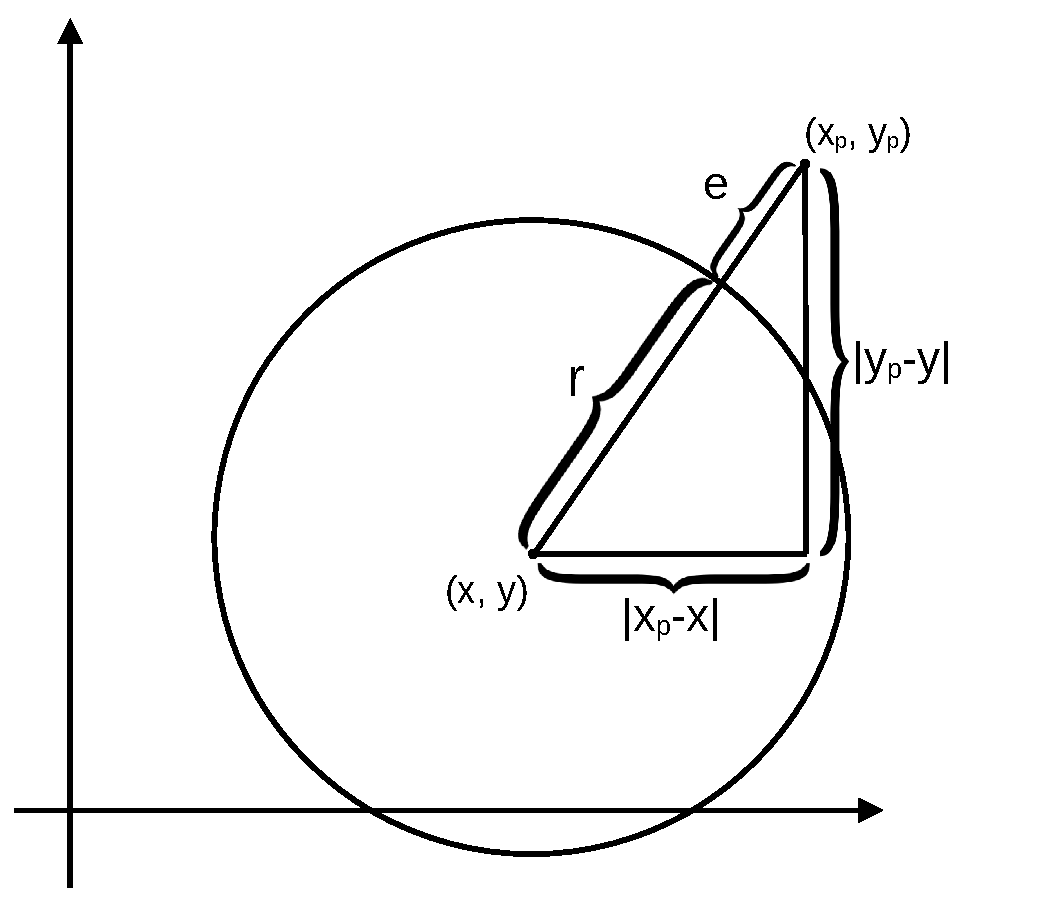
\includegraphics[
            page=1,
            width=220pt,
            height=\textheight,
            keepaspectratio
        ]{Draws/Discesa_del_gradiente_cerchio-punto.pdf}
        \end{center}
        
        \noindent
        Applicando il teorema di pitagora, per differenza, si ottiene che la distanza $ e $ è definita in funzione delle coordinate del centro e del punto in questione, secondo la relazione
        \begin{equation}
             e = \left| \sqrt{(x_p-x)^2 + (y_p-y)^2} -r \right|
        \end{equation}
        
        \noindent
        Possiamo quindi definire la seguente funzione
        \begin{equation}
            f(x, y, r) = \sum_{y_p = 0}^{15} \sum_{x_p = 0}^{15} \left[ g(x_p, y_p) \cdot \left| \sqrt{(x_p-x)^2 + (y_p-y)^2} -r \right| \right] 
        \end{equation}
        
        \noindent
        in cui la funzione $ g(x_p, y_p) $ rappresenta il modulo del gradiente dell'immagine del punto $ (x_p, y_p) $, ed è quindi un coefficiente reale. Tale sommatoria risulta quindi una somma ponderata delle distanze tra la circonferenza in considerazione e tutti i punti della matrice discussa alla sezione precedente. Il modulo del gradiente sarà maggiore per i punti sul contorno dell'immagine del sole, che quindi avranno un peso maggiore rispetto agli altri punti.\\
        Calcoliamo quindi le derivate parziali di $ f(x, y, r) $ rispetto alle tre variabili
        
        \begin {equation}
            \frac{\partial f}{\partial x} = \sum_{y_p = 0}^{15} \sum_{x_p = 0}^{15} \left[ g(x_p, y_p) \cdot sgn \left( \sqrt{(x_p-x)^2 + (y_p-y)^2} - r \right) \cdot \frac{x - x_p}{\sqrt{(x_p - x)^2 + (y_p - y)^2}} \right] 
        \end {equation}
        \begin {equation}
            \frac{\partial f}{\partial y} = \sum_{y_p = 0}^{15} \sum_{x_p = 0}^{15} \left[ g(x_p, y_p) \cdot sgn \left( \sqrt{(x_p-x)^2 + (y_p-y)^2} - r \right) \cdot \frac{y - y_p}{\sqrt{(x_p - x)^2 + (y_p - y)^2}} \right] 
        \end {equation}
        \begin {equation}
            \frac{\partial f}{\partial r} = \sum_{y_p = 0}^{15} \sum_{x_p = 0}^{15} \left[ - g(x_p, y_p) \cdot sgn \left( \sqrt{(x_p-x)^2 + (y_p-y)^2} - r \right) \right] 
        \end {equation}
        
        \noindent
        con $ sgn(x)$ definita a tratti nel dominio $(- \infty ; 0) \cup (0; +\infty) $ :
        
        \begin {equation}
            sgn(x) = 
                \begin{cases}
                  -1 & \text{se x < 0} \\
                  1 & \text{se x > 0}
                \end{cases}
        \end {equation}
        
    \subsection{Esempio di implementazione}

\/*
    \begin{changemargin}{-1cm}{-1cm}

    \lstinputlisting{Sketch_simulazione_elaborato_serra/Sketch_simulazione_elaborato_serra.ino}
    \end{changemargin}
*/    
  
   
    \vfill
    \let\thefootnote\relax\footnotetext{
        \begin{center}
            Documento realizzato in \LaTeX.
        \end{center}
    }
\end{document}

